\documentclass[
	25pt,
	a0paper,
	portrait,
	colspace=15mm,
    blockverticalspace=5mm,
    % margin=25mm
]{tikzposter}

% \renewcommand{\cite}[1]{}

\renewcommand{\familydefault}{\sfdefault}

\usepackage[utf8]{inputenc}
\usepackage{amsmath}

\newcommand{\todo}[1]{{\color{red}#1}}
\newcommand{\TODO}[1]{\textbf{\color{red}[TODO: #1]}}

\newcommand{\paperfontsettings}{
    \renewcommand{\normalsize}{\fontsize{9}{10pt}\selectfont}%
    \renewcommand{\small}{\fontsize{8}{9pt}\selectfont}%
    \renewcommand{\footnotesize}{\fontsize{7}{8pt}\selectfont}%
    \renewcommand{\scriptsize}{\fontsize{6}{8.5pt}\selectfont}%
    \renewcommand{\tiny}{\fontsize{5.5}{6.5pt}\selectfont}%
    \renewcommand{\large}{\fontsize{10}{11pt}\selectfont}%
    \renewcommand{\Large}{\fontsize{11}{11.5pt}\selectfont}%
    \renewcommand{\LARGE}{\fontsize{12}{13pt}\selectfont}%
    \renewcommand{\huge}{\fontsize{14}{14pt}\selectfont}%
    \renewcommand{\Huge}{\fontsize{16}{16pt}\selectfont}%
    \normalsize
}

\newcommand{\figheading}[1]{%
    {\large \textbf{#1}}\\[0.5em]%
}

\usepackage{cleveref}
\usepackage{placeins}
\usepackage{stfloats}
\usepackage{amssymb}
\usepackage{bm}
\usepackage{enumitem}
\usepackage{verbatim}
\usepackage{algorithm}
\usepackage{algpseudocode}
\usepackage{graphicx}

\usepackage{booktabs} 
\usepackage{pgfplots}
\usepackage{url}

\title{BlobBoards: Robust Markers for Accurate Pose}

\author{
    James Pritts
    \quad
    Till Sittart
    \quad
    Hendrik Sauer
    \quad
    Silja Jan\ss{}en
    \quad
    Felix Seegr\"aber
    \quad
    David Nakath
    \quad
    Kevin K\"oser
}

\institute{Marine Data Science, Kiel University}

\definecolor{TFblau}{HTML}{003d86}
\definecolor{CAUpurple}{HTML}{9b0a7d}


\definecolorstyle{TFStyle}{
    \definecolor{colorOne}{named}{TFblau}
    \definecolor{colorTwo}{named}{white}
}{
    \colorlet{backgroundcolor}{white}
	\colorlet{framecolor}{colorOne}
	\colorlet{titlebgcolor}{colorOne}
    \colorlet{titlefgcolor}{white}
	\colorlet{notefgcolor}{black}
    \colorlet{notebgcolor}{colorOne!20}
    \colorlet{notefrcolor}{colorOne}
    \colorlet{blocktitlebgcolor}{colorOne}
    \colorlet{blocktitlefgcolor}{white}
    \colorlet{blockbodybgcolor}{white}
    \colorlet{blockbodyfgcolor}{black}
    \colorlet{innerblocktitlebgcolor}{colorOne}
    \colorlet{innerblocktitlefgcolor}{white}
    \colorlet{innerblockbodybgcolor}{colorOne!10}
    \colorlet{innerblockbodyfgcolor}{black}
}

\usetheme{Desert}
\usecolorstyle{TFStyle}
\usetitlestyle{VerticalShading}

\makeatletter
\settitle{
    \centering
    \makebox[\linewidth]{
        \begin{minipage}{0.1\linewidth}
            \centering
            
\includegraphics[width=\linewidth]{images/logos/kite/PDKiTE_norm_en_blackwhitegrey_SW_v.eps}
        \end{minipage}
        \hfill
		\begin{minipage}{0.55\linewidth}
            \centering
            \color{titlefgcolor} {\Huge \scshape \@title \par}
            \vspace*{1em}
            {\huge \@author \par}
            \vspace*{1em}
            {\LARGE \@institute}
        \end{minipage}
        \hfill
        \begin{minipage}{0.1\linewidth}
            \centering
            
\includegraphics[width=\linewidth]{images/project_page_qr.png}
        \end{minipage}
    }
}
\makeatother

\begin{document}

\maketitle

\begin{columns}
\column{0.5}

\block{Contribution}{
    \begin{center}
        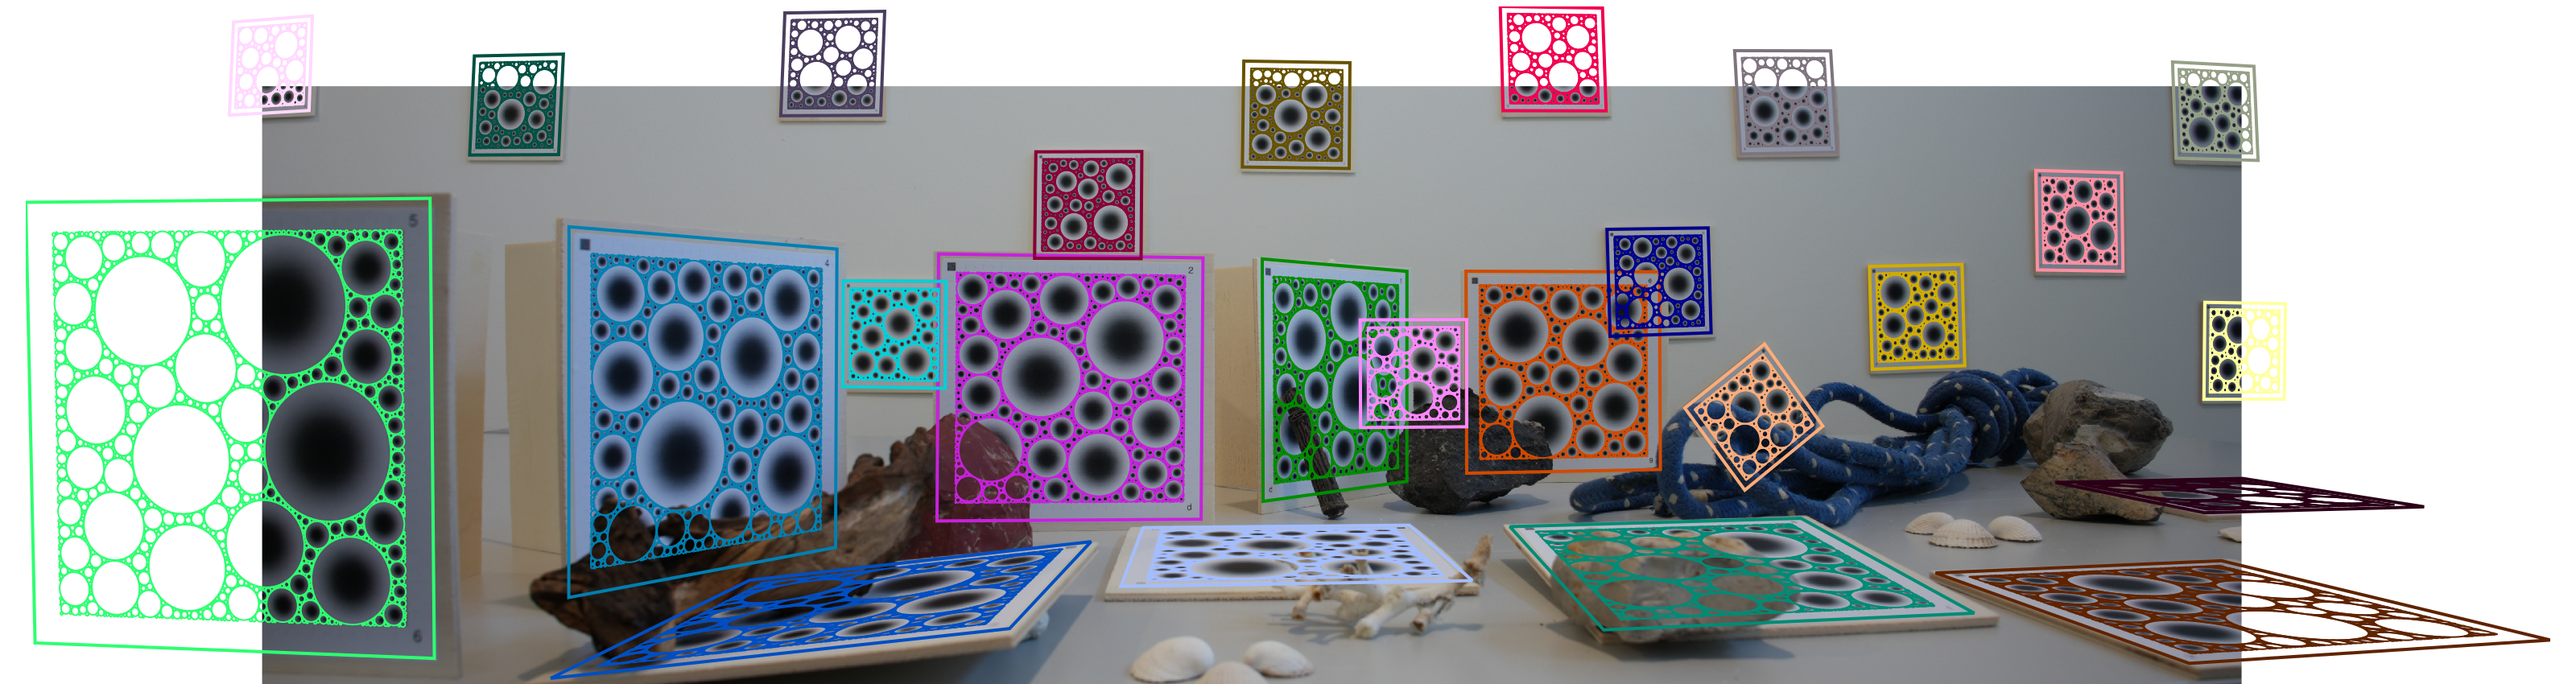
\includegraphics[width=0.9\linewidth]{images/intro_overlay_transparent_background.png}
    \end{center}

    \textbf{Fiducial marker system}
    \begin{itemize}[nosep]
        \item instrinsically multiscale
        \item coverage density for accuracy
        \item robustness against occlusion
    \end{itemize}
}

\block{Why Blobs?}{
    	\begin{center}
    	\begin{minipage}{0.31\linewidth}
    		\centering
    		{\small maximum diameter fraction}\\[2pt]
    		\begin{minipage}{0.31\linewidth}
    			\includegraphics[width=\linewidth]{images/blob_variations_squared/blob_pattern_259_e8a21_co1.5_a1.2_df0.4_s0.2.png}
    		\end{minipage}
    		\hfill
    		\begin{minipage}{0.31\linewidth}
    			\includegraphics[width=\linewidth]{images/blob_variations_squared/blob_pattern_d2d_1c2c0_co1.5_a1.2_df0.5_s0.2.png}
    		\end{minipage}
    		\hfill
    		\begin{minipage}{0.31\linewidth}
    			\includegraphics[width=\linewidth]{images/blob_variations_squared/blob_pattern_714_d3d26_co1.5_a1.2_df0.7_s0.2.png}
    		\end{minipage}
    	\end{minipage}
    	\hfill
    	\begin{minipage}{0.31\linewidth}
    		\centering
    		{\small minimum blob scale}\\[2pt]
    		\begin{minipage}{0.31\linewidth}
    			\includegraphics[width=\linewidth]{images/blob_variations_squared/blob_pattern_259_e8a21_co1.5_a1.2_df0.4_s0.2.png}
    		\end{minipage}
    		\hfill
    		\begin{minipage}{0.31\linewidth}
    			\includegraphics[width=\linewidth]{images/blob_variations_squared/blob_pattern_76a_dc19e_co1.5_a1.2_df0.4_s0.7.png}
    		\end{minipage}
    		\hfill
    		\begin{minipage}{0.31\linewidth}
    			\includegraphics[width=\linewidth]{images/blob_variations_squared/blob_pattern_09f_028f0_co1.5_a1.2_df0.4_s1.7.png}
    		\end{minipage}
    	\end{minipage}
        \hfill
    	\begin{minipage}{0.31\linewidth}
    		\centering
    		{\small support cutoff $c$}\\[2pt]
    		\begin{minipage}{0.31\linewidth}
    			\includegraphics[width=\linewidth]{images/blob_variations_squared/blob_pattern_259_e8a21_co1.5_a1.2_df0.4_s0.2.png}
    		\end{minipage}
    		\hfill
    		\begin{minipage}{0.31\linewidth}
    			\includegraphics[width=\linewidth]{images/blob_variations_squared/blob_pattern_00d_01603_co1.8_a1.2_df0.4_s0.2.png}
    		\end{minipage}
    		\hfill
    		\begin{minipage}{0.3\linewidth}
    			\includegraphics[width=\linewidth]{images/blob_variations_squared/blob_pattern_3af_2509f_co2.0_a1.2_df0.4_s0.2.png}
    		\end{minipage}
    	\end{minipage}
    	% \hfill
    	% \begin{minipage}{0.48\linewidth}
    	% 	\centering
    	% 	{\small scale-sampling distribution}\\[2pt]
    	% 	\begin{minipage}{0.32\linewidth}
    	% 		\includegraphics[width=\linewidth]{images/blob_variations_squared/blob_pattern_259_e8a21_co1.5_a1.2_df0.4_s0.2.png}
    	% 	\end{minipage}
    	% 	\hfill
    	% 	\begin{minipage}{0.32\linewidth}
    	% 		\includegraphics[width=\linewidth]{images/blob_variations_squared/blob_pattern_028_1251d_co1.5_a1.6_df0.4_s0.2.png}
    	% 	\end{minipage}
    	% 	\hfill
    	% 	\begin{minipage}{0.32\linewidth}
    	% 		\includegraphics[width=\linewidth]{images/blob_variations_squared/blob_pattern_4a3_79c86_co1.5_a2.4_df0.4_s0.2.png}
    	% 	\end{minipage}
    	% \end{minipage}
    \end{center}

\begin{itemize}[nosep]
    \item maximises SIFT response
    \item robust to defocus
\end{itemize}
}

\block{Pipeline}{
	% \centering
	\begin{minipage}{0.31\linewidth}
		\centering
		{\small (a) detect}\\[2pt]
		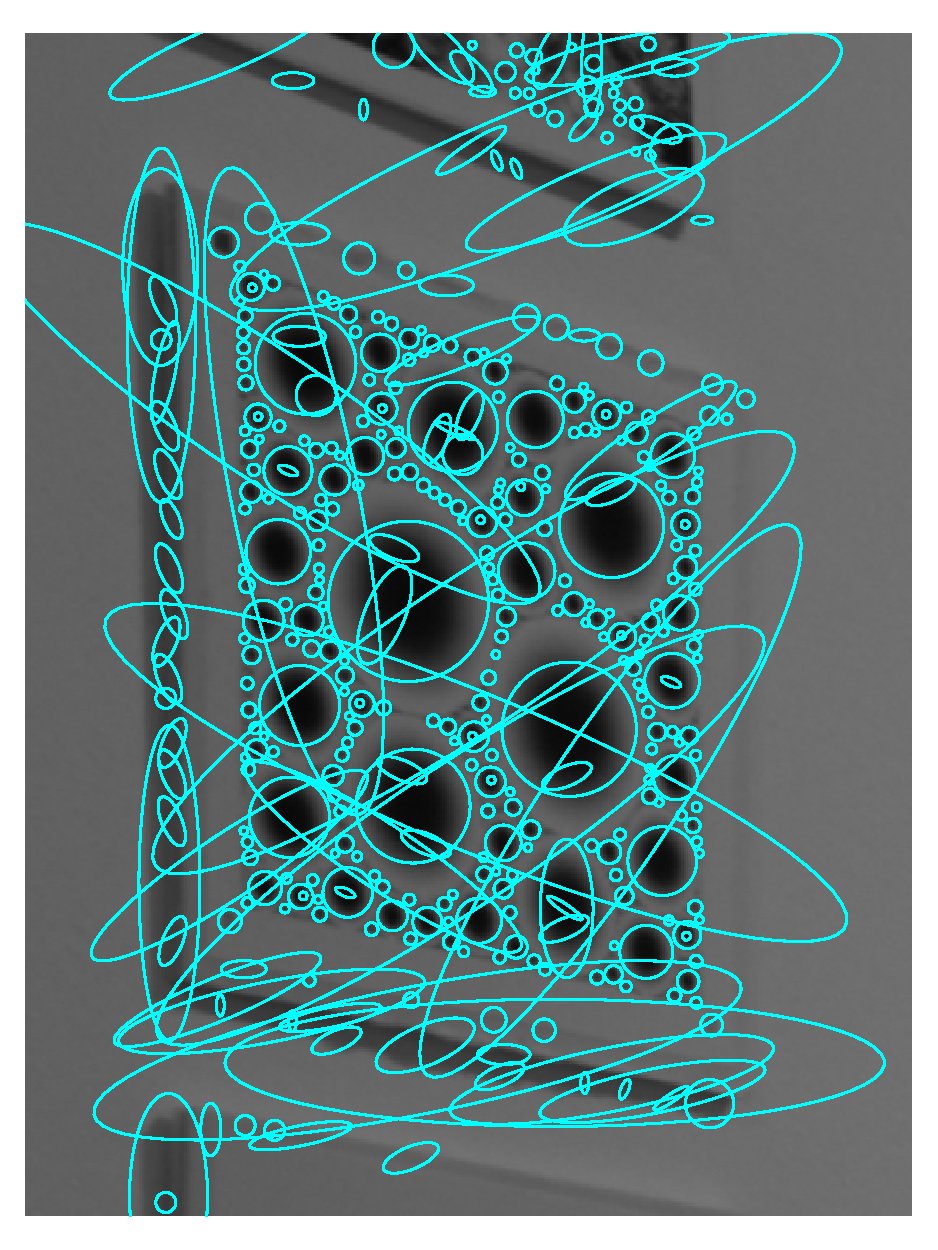
\includegraphics[width=\linewidth]{images/bb_pipe_detect.pdf}
	\end{minipage}\hfill
	\begin{minipage}{0.31\linewidth}
		\centering
		{\small (b) adapt}\\[2pt]
		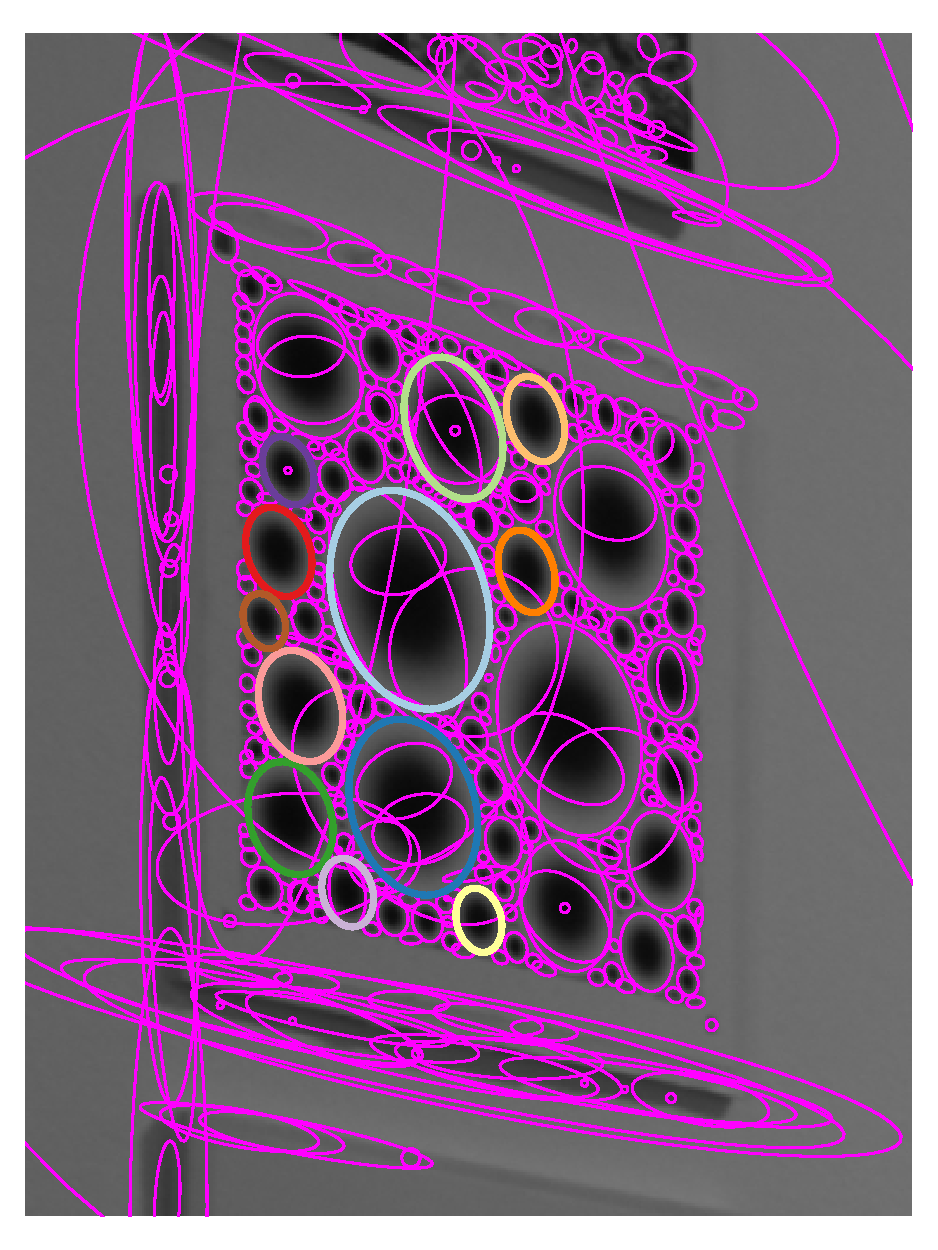
\includegraphics[width=\linewidth]{images/bb_pipe_adapt.pdf}
	\end{minipage}\hfill
	\begin{minipage}{0.31\linewidth}
		\centering
		{\small (c) canonicalize}\\[2pt]
		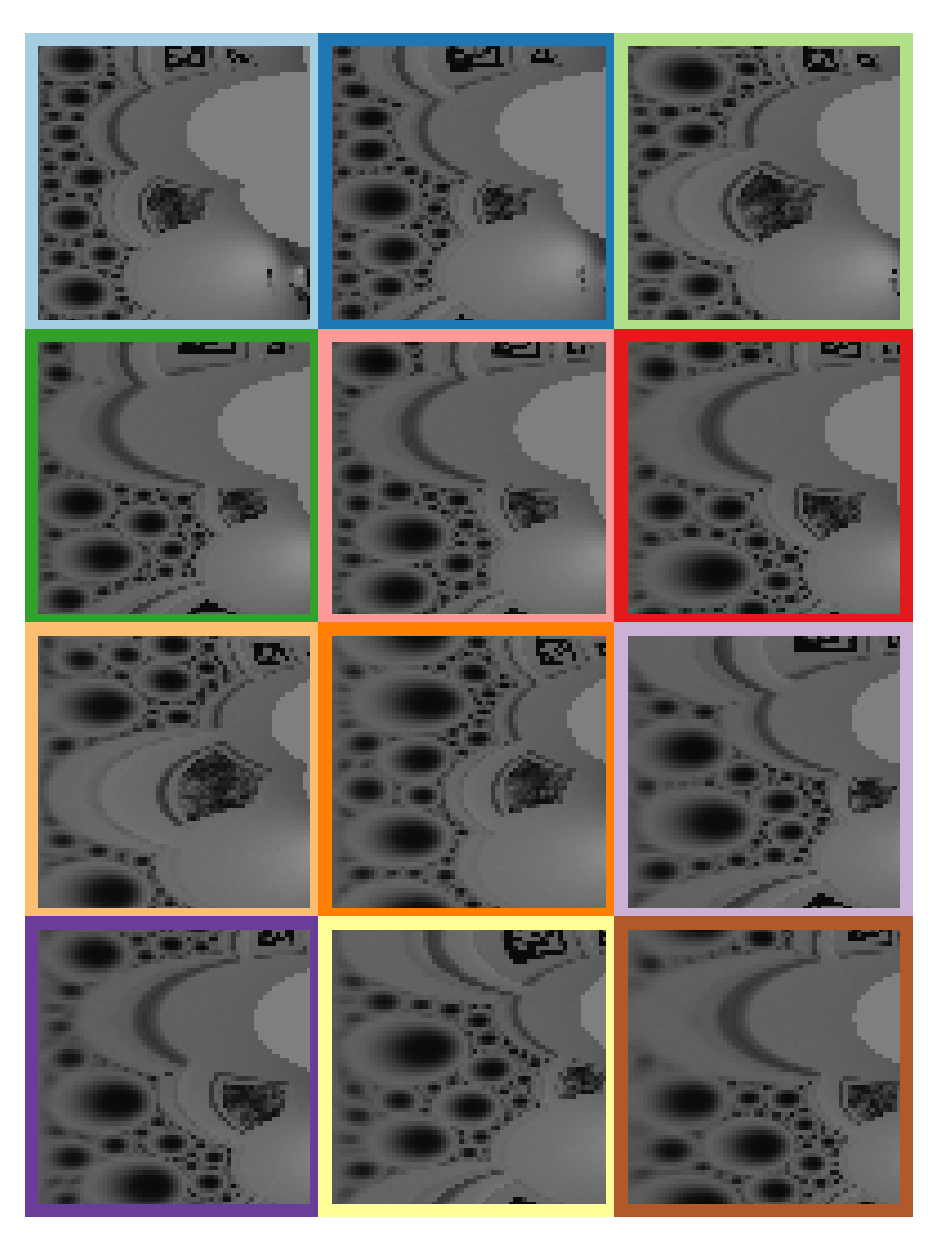
\includegraphics[width=\linewidth]{images/bb_pipe_logpolar.pdf}
	\end{minipage}\\[5pt]

	\begin{minipage}{0.655\linewidth}	% 2x panel width (0.31) + 1x margin width (0.035)
		\centering
		{\small (d) match}\\[2pt]
		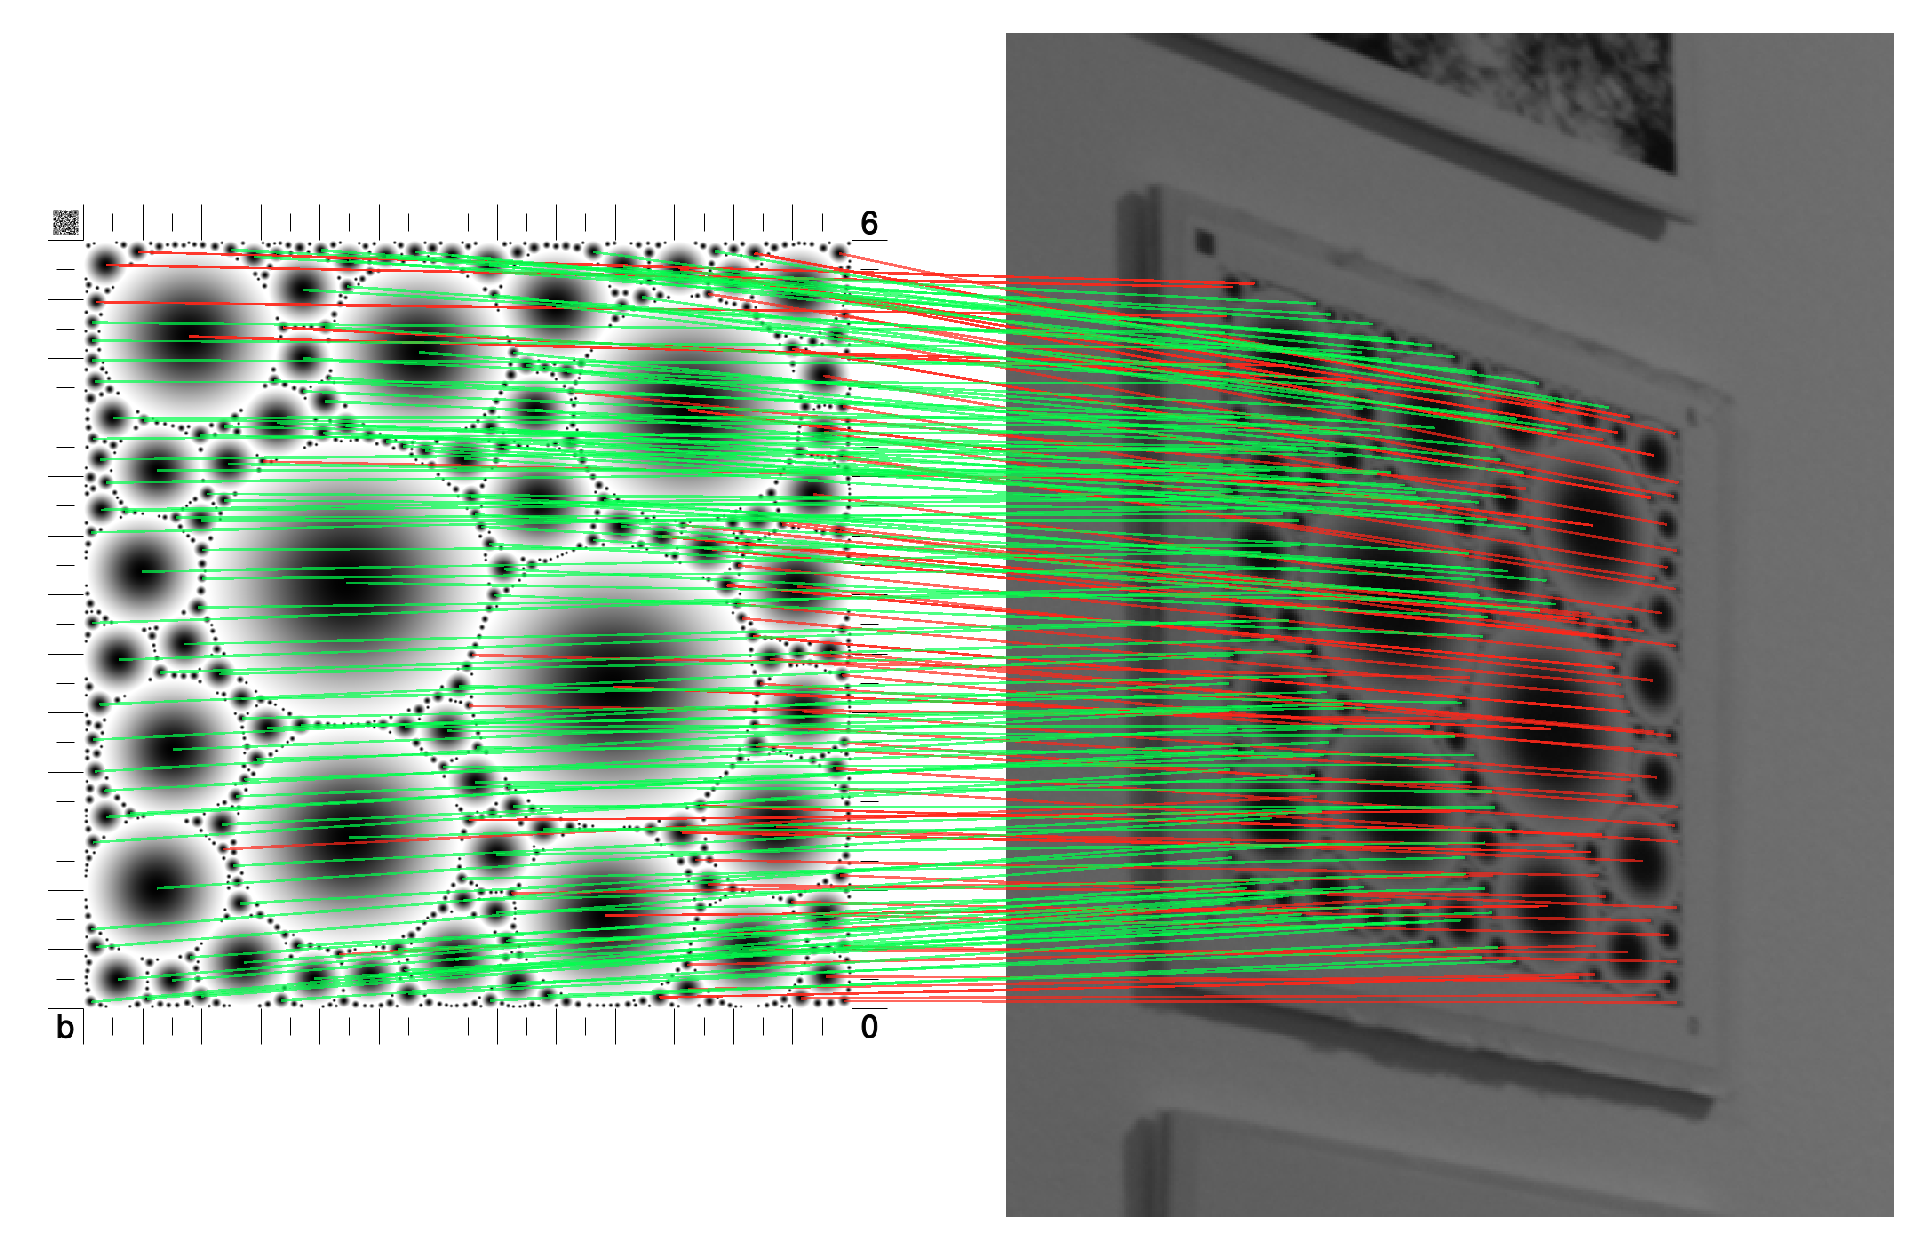
\includegraphics[width=\linewidth]{images/bb_pipe_match.pdf}
	\end{minipage}
	\hfill
	\begin{minipage}{0.31\linewidth}
		\centering
		{\small (e) estimate pose}\\[2pt]
		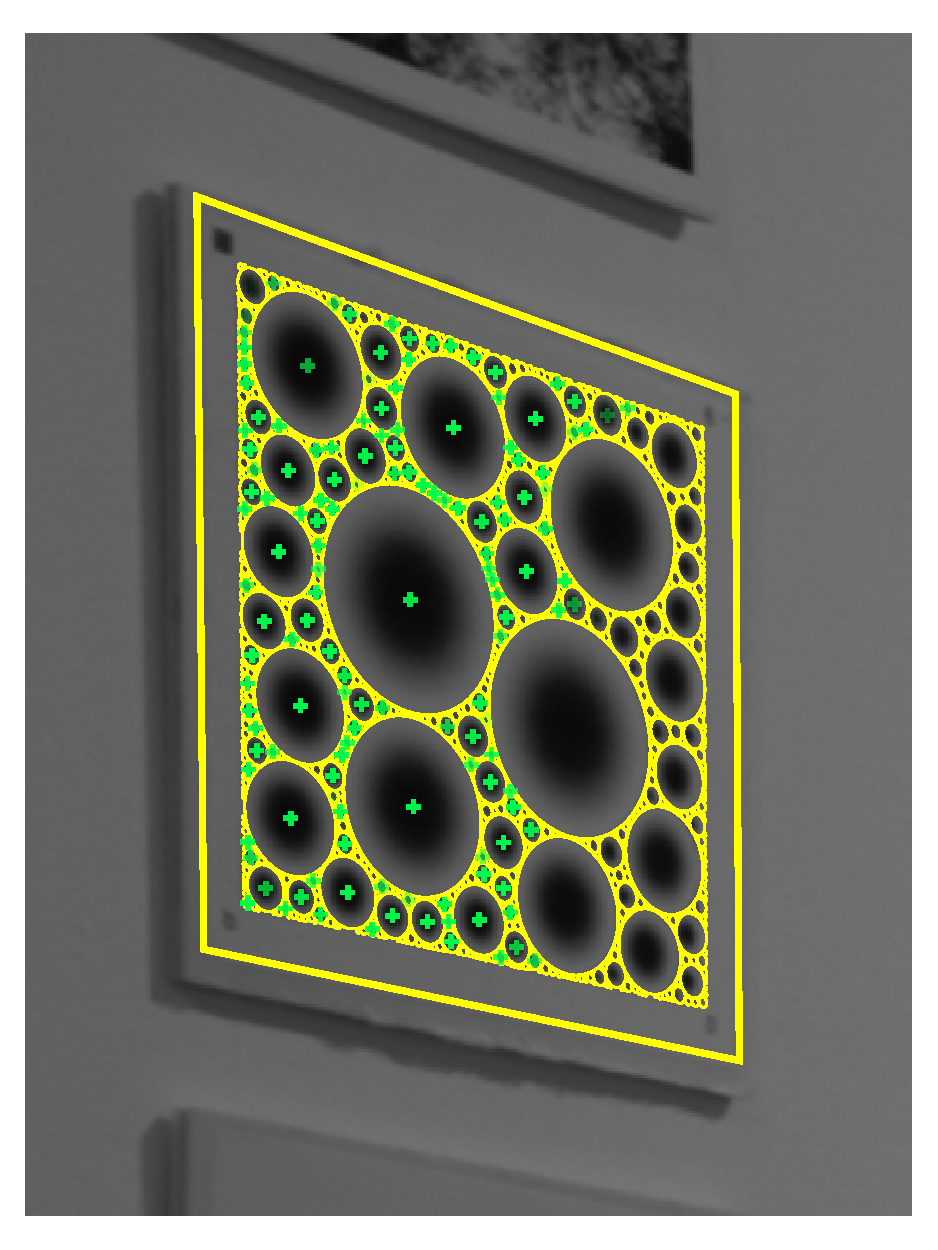
\includegraphics[width=\linewidth]{images/bb_pipe_register.pdf}
	\end{minipage}
}


\block{Experimental Setup}{
	\begin{description}[nosep]
		\item[Setup:] 30 boards at different sizes observed from different distances and view angles
		\item[Baselines:] AprilTag~3 and OpenCV's ArUco detector
		\item[Ground Truth:] motion capture
	\end{description}
	\begin{center}
		\begin{minipage}{0.32\linewidth}
			\centering
			{\small BlobBoards}\\[2pt]
			\includegraphics[width=\linewidth]{images/experiment/bb/DSC04530_val.png}
		\end{minipage}\hfill
		\begin{minipage}{0.32\linewidth}
			\centering
			{\small AprilTag}\\[2pt]
			\includegraphics[width=\linewidth]{images/experiment/apr/DSC04433_val.png}
		\end{minipage}\hfill
		\begin{minipage}{0.32\linewidth}
			\centering
			{\small ArUco}\\[2pt]
			\includegraphics[width=\linewidth]{images/experiment/aru/DSC04343_val.png}
		\end{minipage}
	\end{center}
}

\column{0.5}

\block{Results}{
	\begin{center}
		\begin{minipage}{\linewidth}
			\begin{centering}
				\figheading{p detection and translation error}
				\resizebox{1.05\linewidth}{!}{%
					\paperfontsettings
					\input{figures/floorplan/error_floorplan_ab.tex}
				}
			\end{centering}
		\end{minipage}
	\end{center}
		
	\bigskip
	
	\begin{center}
		\begin{minipage}{\linewidth}
			\begin{centering}
				\figheading{Recall as a function of error}
				\resizebox{1.05\linewidth}{!}{%
					\paperfontsettings
					% error_scale_ecdfs_table.tex — generated assembly; edit freely
\centering
\setlength{\tabcolsep}{2pt}
\providecolor{bbGreen}{HTML}{009E73}
\providecolor{bbBlue}{HTML}{0072B2}
\providecolor{bbOrange}{HTML}{E69F00}
\begin{tabular}{@{}ccc@{}}
{\small Small (4\,cm)} & {\small Medium (6\,cm)} & {\small Large (12\,cm)} \\[1pt]
\input{figures/floorplan/hist_trans_small} & \input{figures/floorplan/hist_trans_medium} & \input{figures/floorplan/hist_trans_large} \\
\multicolumn{3}{c}{(a) Translation error} \\[6pt]
\input{figures/floorplan/hist_rot_small} & \input{figures/floorplan/hist_rot_medium} & \input{figures/floorplan/hist_rot_large} \\
\multicolumn{3}{c}{(b) Rotation error} \\
\\%[4pt]
\multicolumn{3}{c}{
\begin{tikzpicture}[baseline]
\draw[bbBlue, line width=1.2pt] (0.0cm,0) -- (0.6cm,0);
\node[anchor=west, font=\small] at (0.7cm,0) {BlobBoards};
\draw[bbOrange, line width=1.2pt] (3.0cm,0) -- (3.6cm,0);
\node[anchor=west, font=\small] at (3.7cm,0) {AprilTag};
\draw[bbGreen, line width=1.2pt] (6.0cm,0) -- (6.6cm,0);
\node[anchor=west, font=\small] at (6.7cm,0) {ArUco};
\end{tikzpicture}
}
\end{tabular}

				}
			\end{centering}
		\end{minipage}
	\end{center}
    
	% \bigskip
    
	% \begin{center}
    %     \figheading{Planar pose flips (rot error \(> 10\,^\circ\))}
    %     {\small
	% 	\input{figures/floorplan/flip_table.tex}
    %     }
	% \end{center}
}

\block{Occlusion}{
    \begin{description}
        \item[Occlusion Setup:] synthetically occlude boards in 10\,\% increments
    \end{description}

	\bigskip

	\begin{center}
		\begin{minipage}[c]{0.31\linewidth}
			\includegraphics[width=\linewidth]{images/occ_setup/70/compressed_bb_DSC04549.png}
		\end{minipage}\hfill
		\begin{minipage}[c]{0.31\linewidth}
			\includegraphics[width=\linewidth]{images/occ_setup/70/compressed_apr_DSC04451.png}
		\end{minipage}\hfill
		\begin{minipage}[c]{0.31\linewidth}
			\includegraphics[width=\linewidth]{images/occ_setup/70/compressed_uco_DSC04362.png}
		\end{minipage}
	\end{center}

    \bigskip

    \begin{minipage}{\linewidth}
		\begin{center}
			\figheading{p detection for occlusion}
			\resizebox{\linewidth}{!}{%
			\paperfontsettings
			% occlusion_sweep_table.tex — generated assembly; edit freely
\centering
\setlength{\tabcolsep}{2pt}
\providecolor{bbGreen}{HTML}{009E73}
\providecolor{bbBlue}{HTML}{0072B2}
\providecolor{bbOrange}{HTML}{E69F00}
\begin{tabular}{@{}ccc@{}}
\input{figures/floorplan/occ_rot} & \input{figures/floorplan/occ_trans} & \input{figures/floorplan/occ_pod} \\[1pt]
(a) Rotation error & (b) Translation error & (c) Probability of detection \\
% \\[4pt]
\multicolumn{3}{c}{
    \begin{tikzpicture}[baseline]
        \draw[bbBlue, line width=1.2pt] (0.0cm,0) -- (0.6cm,0);
        \node[anchor=west, font=\small] at (0.7cm,0) {BlobBoards};
        \draw[bbOrange, line width=1.2pt] (3.0cm,0) -- (3.6cm,0);
        \node[anchor=west, font=\small] at (3.7cm,0) {AprilTag};
        \draw[bbGreen, line width=1.2pt] (6.0cm,0) -- (6.6cm,0);
        \node[anchor=west, font=\small] at (6.7cm,0) {ArUco};
    \end{tikzpicture}
}

\end{tabular}
			}
		\end{center}
	\end{minipage}
}

\block{Conclusion}{
\begin{center}
	\begin{minipage}[c]{0.19\linewidth}
		\includegraphics[width=\linewidth]{images/adapted/original.jpg}
	\end{minipage}\hfill
	\begin{minipage}[c]{0.19\linewidth}
		\includegraphics[width=\linewidth]{images/adapted/adapted_fde.png}
	\end{minipage}\hfill
	\begin{minipage}[c]{0.19\linewidth}
		\includegraphics[width=\linewidth]{images/adapted/adapted_f80.png}
	\end{minipage}\hfill
	\begin{minipage}[c]{0.19\linewidth}
		\includegraphics[width=\linewidth]{images/adapted/adapted_336.png}
	\end{minipage}\hfill
	\begin{minipage}[c]{0.19\linewidth}
		\includegraphics[width=\linewidth]{images/adapted/adapted_14b.png}
	\end{minipage}
\end{center}
\bigskip
\textbf{Future Work:}
\begin{itemize}
	\item Calibration target
	\item Real-time pose estimation
\end{itemize}
}

\end{columns}

\end{document}
